\section{Future work: integration of DVMS with OpenStack}
\label{sec:future_work}

\subsection{DVMS: a dynamic scheduler for virtual machines}

% \begin{itemize}

% 	\item Dynamic scheduler for virtual machines.

% 	\item Leverage a locality aware p2p overlay.

% 	\item Successfuly tested in simulator (simgrid) and computing grid (grid'5000).

% \end{itemize}

DVMS \cite{quesnel:ispa2013} (Distributed Virtual Machine Scheduler) is a
ressource scheduler that cooperatively and dynamically ensures virtual machines
hosted in large scale infrastructure meet their computing ressources needs. DVMS
treats ressources overloading as a bin packing problem: when a DVMS agent cannot
guarantee its virtual machines needs, it tries to find suitable collaborators 
that will help to make a viable virtual machines placement.

To resolve a ressource overload, a DVMS agent create and join a partition and
forward it to a remote DVMS agent that is not already belonging to a partition.
This remote free agent will first join the partition and then begin to compute 
for a viable mapping. In the case where the computation is unsuccesful, the new 
version of the partition is forwarded to another free DVMS agent until a viable
mapping is found. When a viable mapping has been found, the last member of the
partition applies the mapping by performing live virtual machines migrations.



Formal proof \cite{quesnel:ispa2013} has been made that if a solution exits, 
DVMS will converge to this solution. Furthermore, as a DVMS agent cannot be
shared between different partitions, partitions can work in parallel without
lock mechanisms, thus improving DVMS reactivity. Finally experiments conducted 
on grid5000' testbed have shown that independantly from the infrastructure 
size, partitions only involve few nodes thus limiting the network overhead 
caused by communications.


\subsection{Integration of DVMS in OpenStack}

\label{sub:sec:integration_dvms}

% \begin{itemize}

% \item We propose to replace "nova-scheduler" (static scheduler) by DVMS.

% \item Use of an "Adapter" object that will wrap DVMS and integrate well with OpenStack, as described in figure \ref{fig:integration}
% 	\begin{itemize}
% 		\item It will consume messages that are destinated to "nova-scheduler"

% 		\item Each message will be converted to a "Dvms" message.

% 		\item Each message produced by Dvms will be converted to an OpenStack message and added to the Queue.

% 	\end{itemize}
% \end{itemize}

Section \ref{sub:sec:revisiting_openstack} introduced OpenStack's mechanisms 
that will be revisited. As nova-scheduler currently performs static
ressource scheduling, we decided to replace it by DVMS. Before going more into 
technical details of the integration, OpenStack's service architecture is 
flexible: services follow the "shared nothing memory" principle and communicate
through an AMQP bus. This means that each service follows a "protocol": 
it consummes specific messages received on its queue, performs actions and as a
result produces messages that are sended to collaborators.


This means that if one wants to use a custom service in place of a default 
service, it only have to adapt the custom service to the protocol of the later
one. As all services follow the "shared nothing memory" introduced earlier, if 
the protocol is respected then the system will make no difference between using
the default service or the custom one.

\begin{figure}[h]
	\centering
	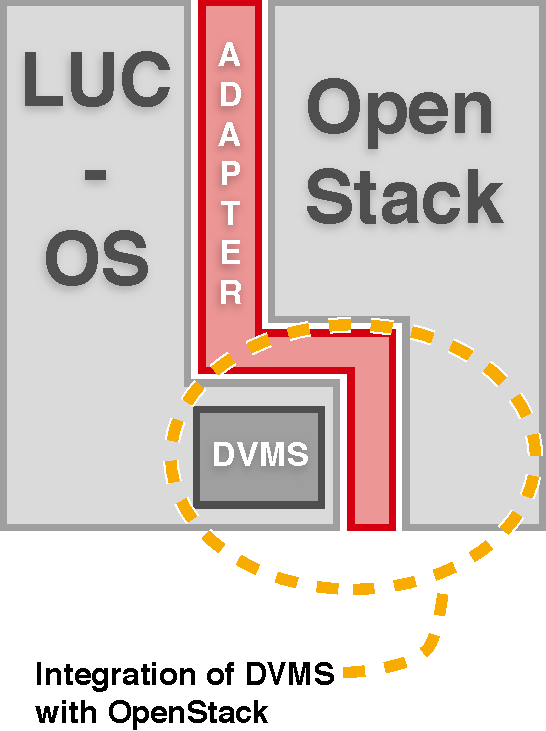
\includegraphics[width=0.50\linewidth]{Figures/dvms_openstack.pdf}
	\caption{Integration of DVMS in OpenStack.}%
	\label{fig:integration}%
	%\vspace*{-.8cm}
\end{figure}

With this in mind, we depicted in figure \ref{fig:integration} the way we plan 
to integrate DVMS with OpenStack: we use an adapter object that consumes 
messages that are destinated to nova-scheduler, forward it to DVMS and translate
messages produced by DMVS in message belonging to the nova-scheduler protocol.
The advantage of this method is that modifications made to the Nova service are
minimized, enabling us to develop a starting prototype of the LUC-OS leveraging
default OpenStack services.

This first prototype will be benchmarked in order to determine what are the
services that are unsuitable with a massively distributed cloud. Depending on 
the results of the benchmark, unsuitable components will be revisited as exposed
in section \ref{sub:sec:revisiting_openstack}.
